% =============================================================================
% 07-linked-lists-doubly-applications-notes.tex — Lecture Notes for Week 7:
% Looking Both Ways (Doubly & Circular Lists, List-Backed Stack and Queue,
% and Polynomials)
%
% DERIVED ARTIFACT. Source of truth:
% Slides/CS301/07-linked-lists-doubly-applications.tex (29 frames incl.
% title/transitions, compiled clean).
% Generated by /lecture-notes at the "textbook-candidate prose" Detail Bar
% (every trace step written out, every example fully solved, Exercises with a
% separate Solutions block, reading guidance per section); do not hand-edit
% content independently of the Beamer source without re-running /qa-notes
% afterward (single-source-of-truth.md).
%
% Page-grounding (inherited 1:1 from the deck header; no upgrades):
%   Karumanchi2017 Ch.3 (Linked Lists, pp.74-162 PDF: doubly/circular),
%   Ch.4 (Stacks, pp.163-204 PDF: linked implementation), Ch.5 (Queues,
%   pp.205-223 PDF: linked implementation); Sedgewick2011 p.142 (linked-list
%   definition), p.120 (stack/queue as collection ADTs); Wirth2004 Sec.4.3
%   (Linear Lists, p.115) for the two-link invariant. Polynomial manipulation
%   is standard treatment: Horowitz & Sahni Ch.4 and Aho-Hopcroft-Ullman Ch.2
%   cited at chapter level only (not page-indexed) -- no page numbers are
%   asserted for it.
%   The Socratic "Delete by pointer" pause and the "Check Your Prediction"
%   frame, plus the three "Before You Go" predictions, are folded into the
%   prose as worked checks carrying the deck's own answers; the Week 6
%   handoff, Week 5 circular-queue cousin, Week 3 stack contract, Week 8
%   searching/sorting, and Week 10 hash-table forward pointers are preserved
%   as stated.
%
% Compile with (Windows/MiKTeX, ';'-joined TEXINPUTS/BIBINPUTS): cd Notes/CS301 &&
%   $env:TEXINPUTS="../../Preambles;"; xelatex -interaction=nonstopmode 07-linked-lists-doubly-applications-notes.tex
%   $env:BIBINPUTS="../..;"; bibtex 07-linked-lists-doubly-applications-notes
%   $env:TEXINPUTS="../../Preambles;"; xelatex -interaction=nonstopmode 07-linked-lists-doubly-applications-notes.tex  (x2)
% =============================================================================

\documentclass[11pt]{article}
\usepackage[margin=1in]{geometry}
% =============================================================================
% Preambles/header.tex — shared LaTeX/Beamer preamble for this project
%
% Use from a Beamer lecture by prepending:
%     \input{header}
% and compiling with TEXINPUTS=../Preambles:$TEXINPUTS (the /compile-latex
% skill does this automatically).
%
% PALETTE CONTRACT. Color names defined here MUST match the names in
% Quarto/theme-template.scss so Beamer and Quarto renderings use the same
% palette. The scripts/check-palette-sync.sh script enforces this.
%
% To customize: edit the HEX values below AND the matching $variable in
% Quarto/theme-template.scss, then run scripts/check-palette-sync.sh.
% =============================================================================

% -----------------------------------------------------------------------------
% Engine detection + encoding
%
% Our /compile-latex skill uses XeLaTeX, where inputenc is unnecessary and
% can produce encoding warnings. Only load inputenc under pdfTeX.
% -----------------------------------------------------------------------------
\usepackage{iftex}
\ifPDFTeX
  \usepackage[utf8]{inputenc}
\fi

\usepackage{amsmath, amssymb, amsthm}
\usepackage{booktabs}
\usepackage{graphicx}

% -----------------------------------------------------------------------------
% PALETTE — mirrors Quarto/theme-template.scss variable names.
% Load xcolor and define colors BEFORE anything that references them
% (notably hyperref, hypersetup, and the Beamer color assignments).
% -----------------------------------------------------------------------------
\usepackage{xcolor}

\definecolor{primary-blue}{HTML}{012169}      % headings, accents
\definecolor{primary-gold}{HTML}{B9975B}      % emphasis, borders
\definecolor{highlight-yellow}{HTML}{F2A900}  % markers, alerts
\definecolor{light-bg}{HTML}{E8EDF5}          % title / section backgrounds
\definecolor{jet}{HTML}{1A1A1A}               % body text

% Semantic colors (used in diagrams and annotations)
\definecolor{positive}{HTML}{15803D}          % good / observed / identified
\definecolor{negative}{HTML}{B91C1C}          % bad / problematic / bias
\definecolor{neutral}{HTML}{525252}           % reference / context

% Highlight accents (match .hi-* classes in the SCSS)
\definecolor{hi-slate}{HTML}{314F4F}
\definecolor{hi-green}{HTML}{2E8B57}
\definecolor{hi-red}{HTML}{C41E3A}

% Semantic aliases so skill templates and snippets can write
% \textcolor{accent}{...} without hard-coding "primary-blue".
\colorlet{accent}{primary-blue}
\colorlet{accent2}{primary-gold}

% -----------------------------------------------------------------------------
% Hyperref — loaded AFTER xcolor + palette so link colors resolve.
% -----------------------------------------------------------------------------
\usepackage{hyperref}
\hypersetup{colorlinks=true, linkcolor=primary-blue, urlcolor=primary-blue,
            citecolor=primary-blue, pdfborder={0 0 0}}

% -----------------------------------------------------------------------------
% Course code — set once per deck (after \input{header}, before \begin{document})
% via \coursecode{CS401}. Shown in the footer on every slide so a deck's course
% is identifiable without opening the title page. Empty by default.
% -----------------------------------------------------------------------------
\makeatletter
\newcommand{\coursecode}[1]{\gdef\@coursecodetext{#1}}
\gdef\@coursecodetext{}
\makeatother

% -----------------------------------------------------------------------------
% Beamer theme assignments (only apply under Beamer).
%
% We detect Beamer via \@ifclassloaded{beamer}, which is the documented,
% non-internal way. This must be wrapped in \makeatletter/\makeatother
% because \@ifclassloaded contains an @-catcode character.
% -----------------------------------------------------------------------------
\makeatletter
\@ifclassloaded{beamer}{%
  \usefonttheme{professionalfonts}
  \setbeamercolor{structure}{fg=primary-blue}
  \setbeamercolor{frametitle}{fg=primary-blue}
  \setbeamercolor{title}{fg=primary-blue}
  \setbeamercolor{subtitle}{fg=primary-gold}
  \setbeamercolor{author}{fg=primary-blue}
  \setbeamercolor{institute}{fg=neutral}
  \setbeamercolor{date}{fg=primary-gold}
  \setbeamercolor{itemize item}{fg=primary-blue}
  \setbeamercolor{itemize subitem}{fg=primary-gold}
  \setbeamercolor{alerted text}{fg=primary-gold}
  \setbeamercolor{block title}{fg=white, bg=primary-blue}
  \setbeamercolor{block body}{bg=light-bg}
  % Semantic block variants: block=definition/concept (blue), exampleblock=
  % worked example (green/positive), alertblock=key takeaway or caution (gold).
  % Keep to <=2 colored boxes per slide across ALL three variants (INV-7).
  \setbeamercolor{block title example}{fg=white, bg=positive}
  \setbeamercolor{block body example}{bg=light-bg}
  \setbeamercolor{block title alerted}{fg=white, bg=primary-gold}
  \setbeamercolor{block body alerted}{bg=light-bg}

  % Minimal footer: course code (left) + page X / N (right), no navigation clutter
  \setbeamertemplate{navigation symbols}{}
  \setbeamertemplate{footline}{%
    \color{neutral}\footnotesize\hspace{0.7em}\@coursecodetext\hfill
    \insertframenumber/\inserttotalframenumber\hspace{0.7em}\vspace{0.3em}}
}{}
\makeatother

% -----------------------------------------------------------------------------
% TikZ setup — libraries the snippet gallery uses
% -----------------------------------------------------------------------------
\usepackage{tikz}
\usetikzlibrary{arrows.meta, positioning, calc, decorations.pathreplacing,
                fit, shapes.geometric, backgrounds}

% Shared TikZ styles — snippets and hand-written diagrams can pick these up
% via `\begin{tikzpicture}[every node/.style={...}]` or by naming specific
% styles (e.g., `\node[dag-node] (X) at (0,0) {X};`).
\tikzset{
  % Node styles for causal DAGs and similar
  dag-node/.style = {
    draw=primary-blue, fill=light-bg, rounded corners=2pt,
    minimum width=1.2cm, minimum height=0.9cm, align=center, font=\small
  },
  decision-node/.style = {
    draw=primary-gold, fill=white, diamond, aspect=1.8,
    minimum width=1.8cm, minimum height=1.2cm, align=center, font=\small,
    inner sep=1pt
  },
  % Edge styles — observed vs counterfactual
  observed-edge/.style = {-{Latex[length=2.5mm]}, thick, draw=jet},
  counterfactual-edge/.style = {-{Latex[length=2.5mm]}, thick, draw=neutral, dashed},
  confound-edge/.style = {-{Latex[length=2.5mm]}, thick, draw=negative, dashed},
  % Data-point styles for plots
  observed-dot/.style = {fill=primary-blue, draw=primary-blue, circle, inner sep=1.2pt},
  counterfactual-dot/.style = {fill=white, draw=neutral, circle, inner sep=1.2pt}
}

% -----------------------------------------------------------------------------
% Convenience macros
% -----------------------------------------------------------------------------
\newcommand{\muted}[1]{\textcolor{neutral}{#1}}
\newcommand{\key}[1]{\textcolor{primary-gold}{\textbf{#1}}}
\newcommand{\good}[1]{\textcolor{positive}{#1}}
\newcommand{\bad}[1]{\textcolor{negative}{#1}}

% Standout frame macro: full-bleed dark background for section transitions.
% Beamer-only (uses \begin{frame}/\setbeamercolor/\usebeamerfont) -- do not
% call from an article-class file (e.g. Notes/<CODE>/*-notes.tex). \muted,
% \key, \good, \bad, and \coursecode above are plain xcolor/gdef and are
% safe to use from either class; verified when Notes/article-class support
% was added.
% Expand: \transitionslide{Your transition title}
\newcommand{\transitionslide}[1]{%
  \begingroup
  \setbeamercolor{background canvas}{bg=primary-blue}
  \begin{frame}[plain]
    \centering
    \vfill
    {\usebeamerfont{title}\color{white}\Large #1\par}
    \vfill
  \end{frame}
  \endgroup
}

% Section divider frame (Beamer-only), an alternative to \transitionslide with a
% darker two-line style: near-black (jet) background, a small white label line
% above a larger gold title, and a thin gold rule along the bottom edge.
% Expand: \sectiondivider{Section 2}{Pointers}
\newcommand{\sectiondivider}[2]{%
  \begingroup
  \setbeamercolor{background canvas}{bg=jet}
  \begin{frame}[plain]
    \vspace*{3.0cm}
    {\color{white}\ttfamily\large #1\par}
    \vspace{0.5cm}
    {\color{primary-gold}\LARGE #2\par}
    \begin{tikzpicture}[remember picture, overlay]
      \draw[primary-gold, line width=2.5pt]
        ($(current page.south west)+(0,0.1)$) -- ($(current page.south east)+(0,0.1)$);
    \end{tikzpicture}
  \end{frame}
  \endgroup
}

% -----------------------------------------------------------------------------
% Channel watermark — "Concepts That Click" (YouTube).
%
% Article-class files (CompetitiveExam Q/A sets, Notes, Assignments) get a
% light diagonal draft watermark on every page plus a centered footer naming
% the channel. Beamer decks get a subtle TikZ background watermark instead
% (the footline already carries the course code). Centralized here so every
% MCQ PDF is branded without per-file edits.
% -----------------------------------------------------------------------------
\makeatletter
\@ifclassloaded{article}{%
  \usepackage{draftwatermark}
  \SetWatermarkText{Concepts That Click}
  \SetWatermarkScale{1}
  \SetWatermarkFontSize{2cm}
  \SetWatermarkLightness{0.86}
  \SetWatermarkAngle{45}
  \usepackage{fancyhdr}
  \pagestyle{fancy}
  \fancyhf{}
  \fancyfoot[C]{\footnotesize\textcolor{neutral}{Concepts That Click~|~YouTube: \href{https://www.youtube.com/@concepts.thatclick}{@concepts.thatclick}}}
  \renewcommand{\headrulewidth}{0pt}
  \renewcommand{\footrulewidth}{0pt}
  \fancypagestyle{plain}{%
    \fancyhf{}%
    \fancyfoot[C]{\footnotesize\textcolor{neutral}{Concepts That Click~|~YouTube: \href{https://www.youtube.com/@concepts.thatclick}{@concepts.thatclick}}}%
    \renewcommand{\headrulewidth}{0pt}%
    \renewcommand{\footrulewidth}{0pt}%
  }
}{}
\@ifclassloaded{beamer}{%
  \setbeamertemplate{background}{%
    \begin{tikzpicture}[remember picture, overlay]
      \node[rotate=45, opacity=0.055, align=center]
        at (current page.center)
        {\Huge\textcolor{neutral}{Concepts That Click}};
    \end{tikzpicture}%
  }
}{}
\makeatother 
\coursecode{CS301}

% Chapter-style numbering: this is Week 7's chapter.
\renewcommand{\thesection}{7.\arabic{section}}
\renewcommand{\thefigure}{7.\arabic{figure}}
\newtheorem{example}{Example}[section]

\newenvironment{definitionbox}[1]{%
  \par\noindent\textbf{Definition (#1).}\ \itshape
}{\par\vspace{0.3em}}

\title{Looking Both Ways\\\large Lecture Notes --- Week 7: Doubly \& Circular Lists, List-Backed Stack and Queue, and Polynomials}
\author{Auqib Hamid Lone\\[0.3em]
  \small Department of Computer Science \& Engineering\\
  \small Government College of Engineering \& Technology (GCET), Ganderbal}
\date{\today}

\begin{document}
\maketitle

\section{Why This Week Exists: What a Backward Link Buys}

\textbf{Read alongside:} Karumanchi, \textit{Data Structures and Algorithms Made Easy}, Ch.~3, pp.74--162 (PDF) --- doubly and circular lists; Wirth, \textit{Algorithms and Data Structures}, Sec.~4.3, p.~115 --- the linear-list links and the invariant that keeps them agreeing.

Four questions organize this chapter, stated here exactly as the deck states them: what does a backward link (\texttt{p->prev}) buy that one link cannot; when a chain has no \texttt{NULL}, where does a walk stop; can the \emph{same} stack and queue contracts run on chains instead of arrays; and why does $5x^{100} + 3x^{2} + 1$ want three nodes rather than 101 array slots. Compressed to a plan: price the backward link, meet the ring, re-implement the stack and queue on chains, then spend linked lists on the syllabus's polynomial.

The handoff from Week~6 is exact. Week~6 built the singly linked list: a node is data plus one link, \texttt{head} is the sole entry, and \texttt{NULL} terminates the chain. Front-insert is $O(1)$ worst case; end-insert, delete, and search are $O(n)$ worst case; the three-pointer reverse runs in $O(n)$ time and $O(1)$ space. It closed on one promise --- ``what does a backward link buy?'' --- and named Week~7 as doubly and circular lists, the list-based stack and queue, and polynomials. The deficiency it left behind is the whole motivation: \emph{every} delete paid the walk, because to unlink a node we first had to find its predecessor. New symbols today are the predecessor link \texttt{p->prev}, the queue's last-node handle \texttt{tail}, and the circular-list conventions (\texttt{last->next == head}; no \texttt{NULL}).

The calculator pipeline makes the need concrete again. The expression processor's symbol table is a linked list of identifiers (Week~6). When a block scope exits, the compiler must delete every identifier declared in it --- and it already holds a pointer to each one, not to its predecessor. Singly, ``delete by pointer'' still costs a walk to find the node whose \texttt{next} points at the target: $O(n)$ worst case, re-finding information we already had. The same need recurs everywhere: text-editor undo/redo, browser back and forward, OS free-lists of memory blocks, and LRU caches. Two arc notes close the framing. Week~5's circular queue advanced an index by $(\texttt{rear} + 1) \bmod n$; today the same wraparound appears as a linked ring. And Week~10 will replay this very symbol table as a hash table, $O(n)$ as a list against $O(1)$ expected hashed. \muted{The course design principle fires again: every structure answers a deficiency the previous one just exhibited --- Week~6's singly list had no backward walk, and the doubly linked list is the fix.}

\section{Doubly Linked Lists: The Second Link and Its Price}

\textbf{Read alongside:} Karumanchi, Ch.~3, pp.74--162 (PDF) --- the doubly-linked node and its insert/delete pointer surgery; Wirth, Sec.~4.3, p.~115 --- the two-link invariant a correct operation must restore.

\subsection{The node that looks both ways}

A user clicks \emph{delete} on a bookmark, and the program holds a pointer straight to that node. Singly, the only way to unlink it is to find the node whose \texttt{next} points at it --- a full walk, $O(n)$ worst case. The work is avoidable: at deletion we can already reach the node, so we should be able to reach its neighbours too. The fix costs exactly one extra pointer per node: store the predecessor as well as the successor.

\begin{definitionbox}{Doubly linked list (Karumanchi Ch.~3, pp.74--162 PDF; Wirth Sec.~4.3, p.~115)}
A \key{doubly linked list} (DLL) is a chain of nodes, each holding data plus \emph{two} links: \texttt{next} to the successor and \texttt{prev} to the predecessor. \texttt{head} points to the first node; the first node's \texttt{prev} is \texttt{NULL} and the last node's \texttt{next} is \texttt{NULL}. \cite{Karumanchi2017_data_structures_algorithms_made_easy,Wirth2004_algorithms_data_structures}
\end{definitionbox}

\noindent In C the node is:
\begin{center}
{\small \texttt{struct node \{ int data; struct node *prev; struct node *next; \};}}
\end{center}

Figure~\ref{fig:dll-node} draws the anatomy. A boxed \texttt{prev}-field sits to the left and a boxed \texttt{next}-field to the right of the \texttt{data} field (drawn holding 42); the whole node is flanked by its predecessor box on the left and its successor box on the right, joined by two-headed arrows. A blue \texttt{p} arrow points at the data field, and the labels \texttt{p->prev} and \texttt{p->next} name the two moves the node now offers. One node therefore offers \emph{two} constant-time moves --- forward through \texttt{p->next} and backward through \texttt{p->prev} --- and that is all the second link does, and all the delete fix needs.

\begin{figure}[h]
  \centering
  % Diagram: doubly-linked node anatomy -- a prev|data|next node between
  % its predecessor and successor. Coordinates: L at (-3.4,0) predecessor;
  % pv at (-1.4,0); da at (0,0) the data p points to; nx at (1.4,0);
  % R at (3.4,0) successor.
  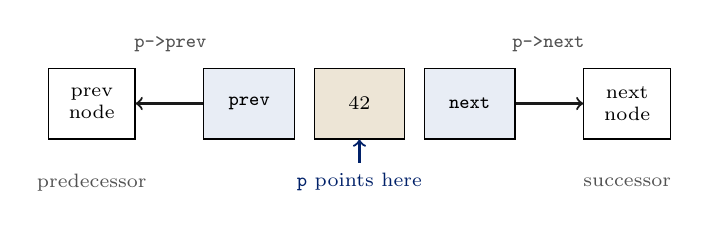
\begin{tikzpicture}[every node/.style={font=\scriptsize}]
    \node[draw, fill=white, minimum width=1.1cm, minimum height=0.9cm,
      align=center] (L) at (-3.4, 0) {prev\\node};
    \node[draw, fill=light-bg, minimum width=1.15cm, minimum height=0.9cm,
      align=center] (pv) at (-1.4, 0) {\texttt{prev}};
    \node[draw, fill=primary-gold!25, minimum width=1.15cm,
      minimum height=0.9cm, align=center] (da) at (0, 0) {42};
    \node[draw, fill=light-bg, minimum width=1.15cm, minimum height=0.9cm,
      align=center] (nx) at (1.4, 0) {\texttt{next}};
    \node[draw, fill=white, minimum width=1.1cm, minimum height=0.9cm,
      align=center] (R) at (3.4, 0) {next\\node};
    \draw[<-, thick, color=jet] (L.east) -- (pv.west);
    \draw[->, thick, color=jet] (nx.east) -- (R.west);
    \node[text=neutral] at (-3.4, -1.0) {predecessor};
    \node[text=neutral] at (3.4, -1.0) {successor};
    \node[text=primary-blue] at (0, -1.0) {\texttt{p} points here};
    \draw[->, thick, color=primary-blue] (0, -0.75) -- (da.south);
    \node[text=neutral] at (-2.4, 0.75) {\texttt{p->prev}};
    \node[text=neutral] at (2.4, 0.75) {\texttt{p->next}};
  \end{tikzpicture}
  \caption{A doubly-linked node: data flanked by \texttt{prev} and \texttt{next} fields, reachable forward and backward in $O(1)$ from a pointer \texttt{p} (cf.\ Karumanchi, Ch.~3, pp.74--162 PDF).}
  \label{fig:dll-node}
\end{figure}

\begin{example}[Worked example: building 10 $\leftrightarrow$ 20 $\leftrightarrow$ 30]
Start empty (\texttt{head} $=$ \texttt{NULL}). Build the chain term by term, each term one \texttt{malloc} plus link repairs whose count is the price of the second pointer. Insert 10 at the front: the new box gets \texttt{prev} $=$ \texttt{NULL}, \texttt{next} $=$ \texttt{NULL}, and \texttt{head} swings onto it --- two link writes. Insert 20 at the front: the new box's \texttt{next} points at the old first node (10) and its \texttt{prev} to \texttt{NULL}; then the old first node's \texttt{prev} must be repointed from \texttt{NULL} to the new box; then \texttt{head} swings over --- three link writes, because an interior neighbour had to be repaired. Insert 30 at the end: walk to the old last node (20), set the fresh 30-box's \texttt{prev} to it and \texttt{next} to \texttt{NULL}, then set the old last node's \texttt{next} to the fresh box --- again an interior-neighbour repair. Final heap: \texttt{head} $\leftrightarrow$ \texttt{[10]} $\leftrightarrow$ \texttt{[20]} $\leftrightarrow$ \texttt{[30]}, where each \texttt{<->} is two links. The bill is exact: one extra pointer per node, and every insert or delete must repair \emph{two} links instead of one.
\end{example}

\subsection{Insert at the front, end, and after a given node}

Pointer surgery for inserting \texttt{x} after a given node \texttt{p} (Karumanchi Ch.~3, pp.74--162 PDF):

{\footnotesize
\begin{verbatim}
newNode = malloc(sizeof(struct node)); newNode->data = x
newNode->next = p->next                 // 1. wire forward
newNode->prev = p                       // 2. wire backward
if (p->next != NULL) p->next->prev = newNode  // 3. fix old successor
p->next = newNode                       // 4. splice in
\end{verbatim}
}

Each step is load-bearing. Step~1 gives the new node its successor --- the old \texttt{p->next} --- while that value is still readable. Step~2 gives it its predecessor, \texttt{p} itself. Step~3 repairs the old successor's backward link so that it now points at the new node; it is guarded by \texttt{p->next != NULL} because if \texttt{p} was the last node there is no successor to repair. Step~4 finally overwrites \texttt{p->next}: order matters here exactly as it did in Week~6's front-insert, because step~3 still needs the old successor value that step~4 destroys. Front-insert and end-insert are the special cases: front-insert sets \texttt{newNode->prev = NULL} and moves \texttt{head}; end-insert is just ``insert after the old last node.''

\begin{definitionbox}{The two-link invariant (Wirth Sec.~4.3, p.~115; standard treatment)}
After any operation, every interior node \texttt{p} satisfies \texttt{p->next->prev == p} \emph{and} \texttt{p->prev->next == p}. Every operation must restore this before it returns.
\end{definitionbox}

Steps~3 and~4 above are precisely what keep the invariant. If you wire \texttt{p->next = newNode} but forget \texttt{p->next->prev = newNode}, then the old successor still points \emph{backward} at \texttt{p}, and the two links silently disagree; a later backward walk either skips the new node or corrupts the chain. The invariant is the single condition that certifies a DLL operation is correct.

Figure~\ref{fig:dll-insert} shows the final state after inserting a gold new node \texttt{X} (holding 20) between \texttt{A} (10) and \texttt{B} (30). Reading the four pointer writes off the picture: \texttt{X->next = B}, \texttt{X->prev = A}, then \texttt{B->prev = X} and \texttt{A->next = X}. The old \texttt{A} $\leftrightarrow$ \texttt{B} link has been overwritten by the pair of two-headed arrows through \texttt{X}; the lesson the diagram encodes is to wire the new node \emph{before} repointing its neighbours --- switch the order and either \texttt{A}'s or \texttt{B}'s neighbour address is lost.

\begin{figure}[h]
  \centering
  % Diagram: final state after inserting new node X (20) between A (10)
  % and B (30) in a doubly linked list. Coordinates: hd label (-4.2,0);
  % A (-2.4,0); X (0,0); B (2.4,0); NL (4.4,0).
  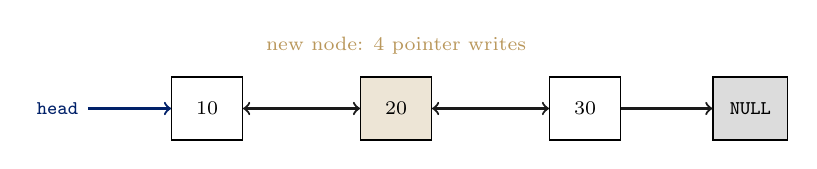
\begin{tikzpicture}[every node/.style={font=\scriptsize}]
    \node[text=primary-blue] (hd) at (-4.3, 0) {\texttt{head}};
    \node[draw, fill=white, minimum width=0.9cm, minimum height=0.8cm,
      align=center] (A) at (-2.4, 0) {10};
    \node[draw, fill=primary-gold!25, minimum width=0.9cm,
      minimum height=0.8cm, align=center] (X) at (0, 0) {20};
    \node[draw, fill=white, minimum width=0.9cm, minimum height=0.8cm,
      align=center] (B) at (2.4, 0) {30};
    \node[draw, fill=neutral!20, minimum width=0.95cm,
      minimum height=0.8cm, align=center] (NL) at (4.5, 0) {\texttt{NULL}};
    \draw[->, thick, color=primary-blue] (hd.east) -- (A.west);
    \draw[<->, thick, color=jet] (A.east) -- (X.west);
    \draw[<->, thick, color=jet] (X.east) -- (B.west);
    \draw[->, thick, color=jet] (B.east) -- (NL.west);
    \node[text=primary-gold] at (0, 0.8) {new node: 4 pointer writes};
  \end{tikzpicture}
  \caption{Inserting \texttt{X} (20) after \texttt{A} (10): four pointer writes restore both links of the two-link invariant (cf.\ Karumanchi, Ch.~3, pp.74--162 PDF).}
  \label{fig:dll-insert}
\end{figure}

\begin{example}[Worked trace: insert 20 after 10 in \texttt{head} $\leftrightarrow$ 10 $\leftrightarrow$ 30]
\texttt{malloc} the new box and fill \texttt{data} $=$ 20. Step~1: \texttt{X->next} $=$ \texttt{p->next}, where \texttt{p} is the 10-node --- so \texttt{X} now points at 30. Step~2: \texttt{X->prev} $=$ \texttt{p} --- \texttt{X} points backward at 10. Step~3: \texttt{p->next} is 30 (not \texttt{NULL}), so set \texttt{30->prev} $=$ \texttt{X} --- the old successor's backward link now names \texttt{X}. Step~4: \texttt{10->next} $=$ \texttt{X} --- splice complete. Final heap reads \texttt{head} $\leftrightarrow$ 10 $\leftrightarrow$ 20 $\leftrightarrow$ 30, and both halves of the invariant hold: \texttt{20->next->prev} $=$ \texttt{30->prev} $=$ 20, and \texttt{20->prev->next} $=$ \texttt{10->next} $=$ 20. Now the failure mode: swap steps 3 and 4 and step~3 sets \texttt{X->prev} on the wrong node (or reads \texttt{p->next} = \texttt{X}, a self-loop), leaving 30's backward link pointing at 10 forever --- a backward walk from 30 reaches 10 and skips 20 entirely. Four writes, and the order is the whole operation.
\end{example}

\subsection{Delete by pointer: the $O(1)$ bypass}

Deleting the node \texttt{p} points at (Karumanchi Ch.~3, pp.74--162 PDF):

{\footnotesize
\begin{verbatim}
if (p->prev != NULL) p->prev->next = p->next
else head = p->next                 // p was the first node
if (p->next != NULL) p->next->prev = p->prev
free(p)                             // reclaim exactly once
\end{verbatim}
}

\key{Socratic pause, exactly as the deck poses it}: with only \texttt{p} in hand, which two nodes must learn the new link --- and how does each find its neighbour without a walk? The answer is the whole payoff: they are \texttt{p->prev} and \texttt{p->next}, both reachable in $O(1)$ straight from \texttt{p}. The first line stitches \texttt{p->prev} to \texttt{p->next} going forward (guarded because if \texttt{p} is the first node there is no predecessor, and instead \texttt{head} must move forward). The second line stitches \texttt{p->next} back to \texttt{p->prev} (guarded because if \texttt{p} is the last node there is no successor to repair). Then \texttt{free(p)} reclaims exactly once. So delete is $O(1)$ worst case once \texttt{p} is known --- against Week~6's $O(n)$.

Figure~\ref{fig:dll-delete} draws deleting the middle node \texttt{D} (holding 20) from \texttt{A} (10) $\leftrightarrow$ \texttt{D} $\leftrightarrow$ \texttt{B} (30). The two dashed red links (\texttt{A} $\leftrightarrow$ \texttt{D} and \texttt{D} $\leftrightarrow$ \texttt{B}) are the ones that die; one green bypass replaces them, drawn as a curve under the row that jumps from \texttt{A} to \texttt{B}. In pointer terms the bypass is the single line \texttt{p->prev->next = p->next; p->next->prev = p->prev}, after which \texttt{free(p)} returns \texttt{D} to the heap.

\begin{figure}[h]
  \centering
  % Diagram: deleting the middle node D (20) of a DLL -- bypass via prev
  % and next. Coordinates: A (0,0); D (2.4,0) doomed; B (4.8,0).
  \begin{tikzpicture}[every node/.style={font=\scriptsize}]
    \node[draw, fill=white, minimum width=0.9cm, minimum height=0.8cm,
      align=center] (A) at (0, 0) {10};
    \node[draw, fill=negative!15, minimum width=0.9cm, minimum height=0.8cm,
      align=center] (D) at (2.4, 0) {20};
    \node[draw, fill=white, minimum width=0.9cm, minimum height=0.8cm,
      align=center] (B) at (4.8, 0) {30};
    \draw[<->, thick, color=negative, dashed] (A.east) -- (D.west);
    \draw[<->, thick, color=negative, dashed] (D.east) -- (B.west);
    \draw[<->, thick, color=positive] (A.south)
      .. controls (1.2, -1.15) and (3.6, -1.15) .. (B.south);
    \node[text=negative, above=0.2cm of D] {doomed: \texttt{free(p)}};
    \node[text=positive] at (2.4, -1.4)
      {\texttt{p->prev->next = p->next; p->next->prev = p->prev}};
  \end{tikzpicture}
  \caption{Deleting the middle node 20: the two dashed \texttt{<->} links die and one green bypass joins 10 and 30 in both directions (cf.\ Karumanchi, Ch.~3, pp.74--162 PDF).}
  \label{fig:dll-delete}
\end{figure}

\begin{example}[Worked trace: delete 15 from \texttt{head} $\leftrightarrow$ 5 $\leftrightarrow$ 15 $\leftrightarrow$ 25]
Given only a pointer \texttt{p} at the 15-node. First line: \texttt{p->prev} is the 5-node (not \texttt{NULL}), so set \texttt{5->next} $=$ \texttt{p->next} $=$ the 25-node. Second line: \texttt{p->next} is the 25-node (not \texttt{NULL}), so set \texttt{25->prev} $=$ \texttt{p->prev} $=$ the 5-node. Third line: \texttt{free(p)} returns the 15-node to the heap. Final heap: \texttt{head} $\leftrightarrow$ 5 $\leftrightarrow$ 25, and the invariant holds (\texttt{5->next->prev} $=$ \texttt{25->prev} $=$ 5). The two links rewritten were 5's \texttt{next} and 25's \texttt{prev}, both reached in $O(1)$ from \texttt{p} --- no walk, $O(1)$ worst case. Touch \texttt{p} after the \texttt{free} and it is Week~1's dangling pointer; skip the \texttt{free} and the 15-node leaks, invisible because nothing points at it.
\end{example}

\subsection{The full price list}

The invariant is the pricing engine: it explains why some operations got cheaper and some did not. The complete Week~7 bill, every bound naming its operation and its case:

\begin{center}
{\footnotesize
\begin{tabular}{lll}
  \toprule
  \textbf{operation} & \textbf{bound} & \textbf{note} \\
  \midrule
  insert at front & $O(1)$ worst case & 2 writes; order matters \\
  insert after given \texttt{p} & $O(1)$ worst case & given pointer skips the walk \\
  delete given \texttt{p} & $O(1)$ worst case & \key{the backward link's payoff} \\
  insert/delete by value & $O(n)$ worst case & the search dominates \\
  search & $O(n)$ worst / $O(1)$ best & unordered; \texttt{prev} does not help \\
  display forward / backward & $\Theta(n)$ & must visit all $n$ \\
  reverse & $O(n)$ worst, $O(1)$ space & one flip + one \texttt{prev} fix per node \\
  \bottomrule
\end{tabular}}
\end{center}

\muted{Search is unchanged: $O(n)$ worst case and $O(1)$ best case --- the backward link does not help an unordered search, because backward and forward walks cost the same per hop. \texttt{displayBwd} needs a \texttt{tail} handle to start from the end; reverse is Week~6's three-pointer flip plus one \texttt{prev} fix per node.} The lesson is the shape of the table: only the operations handed a node pointer outright become $O(1)$; anything that must \emph{find} a node still pays the linear search, and the second link merely doubles the per-node storage and the per-operation link maintenance.

\section{Circular Linked Lists: Rings With No End}

\textbf{Read alongside:} Karumanchi, Ch.~3, pp.74--162 (PDF) --- circular single and double lists and their traversal termination.

\subsection{A ring with no end}

A round-robin scheduler hands the CPU to each process in turn and then returns to the first; a repeating playlist does the same; so does a token-ring network. The last element is followed by the first --- there is no natural end. A chain that models this should make the last node point back to the first instead of to \texttt{NULL}.

\begin{definitionbox}{Circular linked list (Karumanchi Ch.~3, pp.74--162 PDF)}
A \key{circular linked list} is a chain whose last node's \texttt{next} points back to \texttt{head} instead of \texttt{NULL}. In a \key{singly circular} list each node has one link; in a \key{doubly circular} list \texttt{prev} and \texttt{next} both close the ring (\texttt{head->prev} is the last node). An empty circular list has \texttt{head == NULL}; a one-node circular list points to itself. \cite{Karumanchi2017_data_structures_algorithms_made_easy}
\end{definitionbox}

Figure~\ref{fig:circular} draws the two rings side by side. On the left, three nodes \texttt{a}, \texttt{b}, \texttt{c} sit on a circle joined by one-way arcs, so a walk moves \texttt{a} $\to$ \texttt{b} $\to$ \texttt{c} $\to$ \texttt{a} forever; the annotation records the rule that ``last next $=$ head; no \texttt{NULL}.'' On the right, the same three nodes are joined by two-headed arcs, so a walk moves both ways around the ring; the annotation records that \texttt{prev} and \texttt{next} both close the ring. A blue \texttt{head} arrow enters each ring at node \texttt{a}. The picture's point is that a ring has no terminus to draw --- so the walk must name a node to stop on.

\begin{figure}[h]
  \centering
  % Diagram: two rings -- singly circular (left, one-way arcs) and doubly
  % circular (right, two-way arcs). Coordinates: singly nodes sA/sB/sC at
  % angles 90/210/330 on radius 1.25 around (-3,0); doubly dA/dB/dC around
  % (3,0). Arcs drawn at radius 1.25/1.32 between node gaps.
  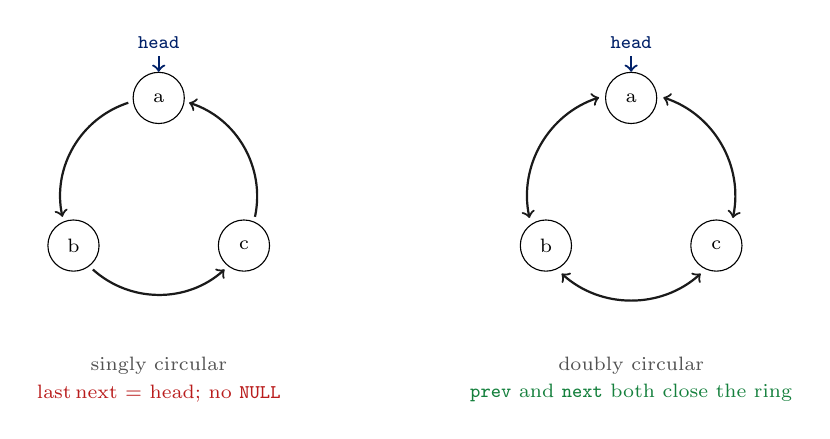
\begin{tikzpicture}[every node/.style={font=\scriptsize}]
    \begin{scope}[shift={(-3,0)}]
      \node[draw, circle, fill=white, minimum size=0.65cm, inner sep=0]
        (sA) at (90:1.25) {a};
      \node[draw, circle, fill=white, minimum size=0.65cm, inner sep=0]
        (sB) at (210:1.25) {b};
      \node[draw, circle, fill=white, minimum size=0.65cm, inner sep=0]
        (sC) at (330:1.25) {c};
      \draw[->, thick, color=jet] (108:1.25) arc (108:192:1.25);
      \draw[->, thick, color=jet] (228:1.25) arc (228:312:1.25);
      \draw[->, thick, color=jet] (348:1.25) arc (348:432:1.25);
      \node[text=primary-blue] at (90:1.95) {\texttt{head}};
      \draw[->, thick, color=primary-blue] (90:1.78) -- (sA.north);
      \node[text=neutral] at (0, -2.15) {singly circular};
      \node[text=negative] at (0, -2.5)
        {last$\,$next $=$ head; no \texttt{NULL}};
    \end{scope}
    \begin{scope}[shift={(3,0)}]
      \node[draw, circle, fill=white, minimum size=0.65cm, inner sep=0]
        (dA) at (90:1.25) {a};
      \node[draw, circle, fill=white, minimum size=0.65cm, inner sep=0]
        (dB) at (210:1.25) {b};
      \node[draw, circle, fill=white, minimum size=0.65cm, inner sep=0]
        (dC) at (330:1.25) {c};
      \draw[<->, thick, color=jet] (108:1.32) arc (108:192:1.32);
      \draw[<->, thick, color=jet] (228:1.32) arc (228:312:1.32);
      \draw[<->, thick, color=jet] (348:1.32) arc (348:432:1.32);
      \node[text=primary-blue] at (90:1.95) {\texttt{head}};
      \draw[->, thick, color=primary-blue] (90:1.78) -- (dA.north);
      \node[text=neutral] at (0, -2.15) {doubly circular};
      \node[text=positive] at (0, -2.5)
        {\texttt{prev} and \texttt{next} both close the ring};
    \end{scope}
  \end{tikzpicture}
  \caption{Two rings: a singly circular list (left, one-way arcs, last link home) and a doubly circular list (right, two-way arcs) (cf.\ Karumanchi, Ch.~3, pp.74--162 PDF).}
  \label{fig:circular}
\end{figure}

\subsection{Traversal without \texttt{NULL}}

The termination rule (Karumanchi Ch.~3, pp.74--162 PDF):

{\footnotesize
\begin{verbatim}
p = head
if (p != NULL) do { visit p; p = p->next } while (p != head)
// stop when the walk RETURNS TO HEAD, not when it hits NULL
\end{verbatim}
}

The subtlety is that a \texttt{while (p != NULL)} loop on a circular list never meets \texttt{NULL}: it loops forever or crashes. The stop condition must name \texttt{head}, and it must be checked \emph{after} the first visit (a \texttt{do--while}) so the head node is not skipped --- the loop body runs once, then the test compares against \texttt{head}. For the doubly circular ring the same rule with \texttt{p->prev} walks the ring the other way. A consequence is that every operation ending at the ``last'' node must handle wraparound: insert and delete must keep the ring closed by repairing both \texttt{head->prev} and \texttt{last->next}.

Rings are not a curiosity --- they are exactly what round-robin schedulers, repeating playlists, and token-ring networks need, and the circular queue's modular index is the same idea seen as a linked ring (Week~5's $(\texttt{rear} + 1) \bmod n$ become one link step around the ring).

\begin{example}[Check your prediction: \texttt{while (p != NULL)} on a 4-node ring]
A singly circular list holds four nodes: \texttt{head} $\to$ a $\to$ b $\to$ c $\to$ d $\to$ a. You run \texttt{while (p != NULL) \{ p = p->next; \}}. Options: (A) visits a, b, c, d then stops; (B) loops forever; (C) stops after one node. The deck's answer is \textbf{B}. Option~A would hold only if some \texttt{next} were \texttt{NULL}, but in a ring none is; option~C misreads the loop --- the condition is checked every hop, not once. Because no node ever holds \texttt{NULL}, the test never fires and the walk cycles a, b, c, d, a, b, c, d, \dots\ indefinitely. The fix is to test \texttt{p != head} (or to visit with a \texttt{do--while} so the first node is not skipped).
\end{example}

\section{Stack and Queue, Reborn on Chains}

\textbf{Read alongside:} Karumanchi, Ch.~4, pp.163--204 (PDF) --- the linked stack; Ch.~5, pp.205--223 (PDF) --- the linked queue; Sedgewick \& Wayne, \textit{Algorithms}, Sec.~1.3, p.~120 --- stack and queue as collection ADTs.

\muted{One ADT, implemented twice: the same Week~3 stack contract, now on chains.} The point of this section is that the contract does not change --- only the implementation does, and therefore only the cost profile moves.

\subsection{List-based stack: push and pop at the head}

A stack over a linked list (Karumanchi Ch.~4, pp.163--204 PDF; Sedgewick Sec.~1.3, p.~120):

{\footnotesize
\begin{verbatim}
push(x): newNode = malloc(...); newNode->data = x
         newNode->next = head; head = newNode      // O(1) worst
pop():   if (head == NULL) error                  // stack underflow
         temp = head; head = head->next
         x = temp->data; free(temp); return x      // O(1) worst
\end{verbatim}
}

The top of the stack is \texttt{head}. Reading the code against Week~6: \texttt{push} is exactly Week~6's front-insert, and \texttt{pop} is exactly Week~6's front-delete --- both rewrite one link (plus \texttt{head}), so both are $O(1)$ worst case. The underflow check is the contract's edge case: \texttt{pop} on an empty stack is an error, not a \texttt{NULL}-dereference. The array version (Week~3) was also $O(1)$ per operation; the list's win is unbounded size and no amortized reallocation, at the cost of $O(n)$ space for $n$ items (one node each) and the pointer-chasing locality that comes with it. \cite{Karumanchi2017_data_structures_algorithms_made_easy,Sedgewick2011_algorithms}

Figure~\ref{fig:list-stack} draws a list-based stack. \texttt{head} (blue) enters the gold-filled node 30 --- the top of the stack, since \texttt{top} $=$ \texttt{head} --- which links down to 20, then 10, then \texttt{NULL}. The annotation records that \texttt{push}/\texttt{pop} touch only \texttt{head}, at $O(1)$ worst case. After \texttt{push(40)}, \texttt{head} points at the new 40-node and its \texttt{next} is the old top (30); \texttt{pop} reverses exactly that, returning the old top and freeing its box.

\begin{figure}[h]
  \centering
  % Diagram: list-based stack, top = head. Coordinates: hd label (-4.7,0.6);
  % node 30 (-3.3,0.6); 20 (-1.3,0.6); 10 (0.7,0.6); NULL (2.8,0.6).
  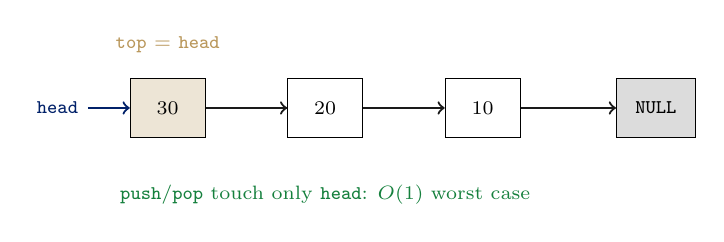
\begin{tikzpicture}[every node/.style={font=\scriptsize}]
    \node[text=primary-blue] (hd) at (-4.8, 0.6) {\texttt{head}};
    \node[draw, fill=primary-gold!25, minimum width=0.95cm,
      minimum height=0.75cm, align=center] (t) at (-3.4, 0.6) {30};
    \node[draw, fill=white, minimum width=0.95cm, minimum height=0.75cm,
      align=center] (m) at (-1.4, 0.6) {20};
    \node[draw, fill=white, minimum width=0.95cm, minimum height=0.75cm,
      align=center] (b) at (0.6, 0.6) {10};
    \node[draw, fill=neutral!20, minimum width=1.0cm,
      minimum height=0.75cm, align=center] (nl) at (2.8, 0.6)
      {\texttt{NULL}};
    \draw[->, thick, color=primary-blue] (hd.east) -- (t.west);
    \draw[->, thick, color=jet] (t.east) -- (m.west);
    \draw[->, thick, color=jet] (m.east) -- (b.west);
    \draw[->, thick, color=jet] (b.east) -- (nl.west);
    \node[text=primary-gold] at (-3.4, 1.4) {\texttt{top} = \texttt{head}};
    \node[text=positive] at (-1.4, -0.5)
      {\texttt{push}/\texttt{pop} touch only \texttt{head}: $O(1)$ worst
      case};
  \end{tikzpicture}
  \caption{A list-based stack: \texttt{head} is the top; \texttt{push} front-inserts and \texttt{pop} front-deletes, both $O(1)$ worst case (cf.\ Karumanchi, Ch.~4, pp.163--204 PDF).}
  \label{fig:list-stack}
\end{figure}

\begin{example}[Worked trace: \texttt{push(40)} then \texttt{pop()} on \texttt{head} $\to$ 30 $\to$ 20 $\to$ 10 $\to$ \texttt{NULL}]
\texttt{push(40)}: \texttt{malloc} a box, set \texttt{data} $=$ 40, set its \texttt{next} $=$ \texttt{head} (the 30-node), then park \texttt{head} on the new box. Heap now reads \texttt{head} $\to$ 40 $\to$ 30 $\to$ 20 $\to$ 10 $\to$ \texttt{NULL}; the top is 40, two pointer writes, $O(1)$ worst case. \texttt{pop()}: \texttt{head} is not \texttt{NULL}, so \texttt{temp} $=$ \texttt{head} (the 40-node), \texttt{head} $=$ \texttt{head->next} (the 30-node), read \texttt{temp->data} $=$ 40, \texttt{free(temp)}, return 40. Heap is back to \texttt{head} $\to$ 30 $\to$ 20 $\to$ 10 $\to$ \texttt{NULL} --- exactly the prior state, showing \texttt{pop} is the precise inverse of \texttt{push}. Called once more on the now-empty stack (all four popped), \texttt{head} is \texttt{NULL} and \texttt{pop} raises underflow instead of dereferencing.
\end{example}

\subsection{List-based queue: keep a tail pointer}

A queue over a linked list (Karumanchi Ch.~5, pp.205--223 PDF; Sedgewick Sec.~1.3, p.~120):

{\footnotesize
\begin{verbatim}
enqueue(x):
  newNode = malloc(...); newNode->data = x
  newNode->next = NULL
  if (head == NULL) head = tail = newNode
  else tail->next = newNode; tail = newNode    // O(1)
dequeue(): if (head == NULL) error      // underflow
           temp = head; head = head->next
           if (head == NULL) tail = NULL
           x = temp->data; free(temp); return x
\end{verbatim}
}

\texttt{enqueue} appends at the \texttt{tail} and advances it: first link the new node after the current last node, then move \texttt{tail} onto it. The empty-list branch sets both \texttt{head} and \texttt{tail} to the single new node. \texttt{dequeue} removes at \texttt{head} --- the oldest element, the one next to leave --- and has one extra guard: if removing the last item empties the queue, \texttt{tail} must be cleared to \texttt{NULL} along with \texttt{head}, or the next \texttt{enqueue} would link onto freed memory. Keeping \texttt{tail} makes end-insert $O(1)$, so both ends are $O(1)$ worst case --- unlike a fixed array. \cite{Karumanchi2017_data_structures_algorithms_made_easy,Sedgewick2011_algorithms}

Figure~\ref{fig:list-queue} draws a list-based queue. \texttt{head} (blue) enters 10, the oldest item; the chain runs 10 $\to$ 20 $\to$ the gold-filled 30, with \texttt{tail} (gold arrow from above) pointing at 30, the newest item; then \texttt{NULL}. The annotations record the two ends: \texttt{dequeue} from \texttt{head}, \texttt{enqueue} after \texttt{tail}. \texttt{enqueue} links after \texttt{tail} and advances it; \texttt{dequeue} unlinks \texttt{head}.

\begin{figure}[h]
  \centering
  % Diagram: list-based queue, dequeue at head, enqueue at tail.
  % Coordinates: hd label (-4.8,0); n1 10 (-3.4,0); n2 20 (-1.3,0);
  % n3 30 (0.8,0) filled gold; NULL (2.8,0); tail label above n3.
  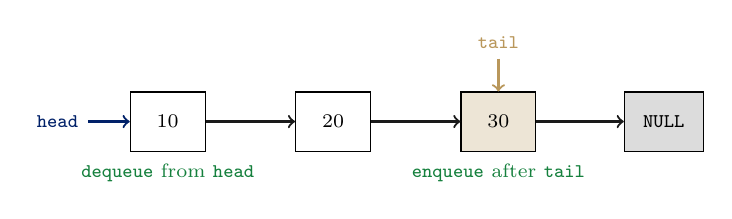
\begin{tikzpicture}[every node/.style={font=\scriptsize}]
    \node[text=primary-blue] (hd) at (-4.9, 0) {\texttt{head}};
    \node[draw, fill=white, minimum width=0.95cm, minimum height=0.75cm,
      align=center] (n1) at (-3.5, 0) {10};
    \node[draw, fill=white, minimum width=0.95cm, minimum height=0.75cm,
      align=center] (n2) at (-1.4, 0) {20};
    \node[draw, fill=primary-gold!25, minimum width=0.95cm,
      minimum height=0.75cm, align=center] (n3) at (0.7, 0) {30};
    \node[draw, fill=neutral!20, minimum width=1.0cm,
      minimum height=0.75cm, align=center] (nl) at (2.8, 0) {\texttt{NULL}};
    \draw[->, thick, color=primary-blue] (hd.east) -- (n1.west);
    \draw[->, thick, color=jet] (n1.east) -- (n2.west);
    \draw[->, thick, color=jet] (n2.east) -- (n3.west);
    \draw[->, thick, color=jet] (n3.east) -- (nl.west);
    \node[text=primary-gold] (tl) at (0.7, 1.0) {\texttt{tail}};
    \draw[->, thick, color=primary-gold] (tl.south) -- (n3.north);
    \node[text=positive] at (-3.5, -0.65)
      {\texttt{dequeue} from \texttt{head}};
    \node[text=positive] at (0.7, -0.65)
      {\texttt{enqueue} after \texttt{tail}};
  \end{tikzpicture}
  \caption{A list-based queue: \texttt{dequeue} unlinks \texttt{head} (oldest), \texttt{enqueue} links after \texttt{tail} (newest); both ends $O(1)$ worst case (cf.\ Karumanchi, Ch.~5, pp.205--223 PDF).}
  \label{fig:list-queue}
\end{figure}

\begin{example}[Worked trace: \texttt{dequeue()} then \texttt{enqueue(40)} on \texttt{head} $\to$ 10 $\to$ 20 $\to$ 30 $\to$ \texttt{NULL}, \texttt{tail} at 30]
\texttt{dequeue()}: \texttt{head} is not \texttt{NULL} (\texttt{temp} $=$ the 10-node), then \texttt{head} $=$ \texttt{head->next} (the 20-node). \texttt{head} is not \texttt{NULL}, so \texttt{tail} stays on 30. Read 10, \texttt{free} the 10-node, return 10. Heap: \texttt{head} $\to$ 20 $\to$ 30 $\to$ \texttt{NULL}, \texttt{tail} still 30. \texttt{enqueue(40)}: \texttt{malloc} a box with \texttt{data} 40 and \texttt{next} \texttt{NULL}; \texttt{head} is not \texttt{NULL}, so \texttt{tail->next} (30's next) $=$ 40, then \texttt{tail} $=$ the 40-node. Heap: \texttt{head} $\to$ 20 $\to$ 30 $\to$ 40 $\to$ \texttt{NULL}, \texttt{tail} now 40. Now the emptying case: from \texttt{head} $\to$ 20 $\to$ \texttt{NULL} with \texttt{tail} on 20, \texttt{dequeue()} sets \texttt{head} $=$ \texttt{NULL} and then, because the new \texttt{head} is \texttt{NULL}, also sets \texttt{tail} $=$ \texttt{NULL} --- without that guard, the next \texttt{enqueue} would write through a stale \texttt{tail} into freed memory.
\end{example}

\subsection{Array vs.\ list: the honest bill}

\begin{center}
{\footnotesize
\begin{tabular}{lll}
  \toprule
  \textbf{operation} & \textbf{array} & \textbf{linked list} \\
  \midrule
  stack \texttt{push}/\texttt{pop} & $O(1)$ worst, fixed capacity$^{*}$ & $O(1)$ worst, unbounded \\
  queue \texttt{enqueue}/\texttt{dequeue} & $O(1)$ worst (circular), fixed & $O(1)$ worst (\texttt{head}+\texttt{tail}), unbounded \\
  memory & one block of $n$ slots & one node per item, +1 pointer each \\
  locality & contiguous, cache-friendly & scattered, pointer-chasing \\
  \bottomrule
\end{tabular}}
\end{center}

\noindent $^{*}$Stack reallocation is amortized $O(1)$ when it grows. There is no universal winner: choose the array when the size is known or bounded and locality matters; choose the list when the size is unpredictable and growth is frequent. The contract is identical --- only the cost profile moves, which is exactly the abstraction the ADT was supposed to give us.

\muted{Circular-queue variant: keeping \texttt{tail->next == head} closes the ring, so one \texttt{tail} pointer gives round-robin \texttt{enqueue} and \texttt{dequeue} at $O(1)$ worst case --- no \texttt{count}, no sacrificed slot, no \texttt{mod} (Week~5's linked cousin). The single handle \texttt{tail} reaches the front through \texttt{tail->next}, so both the enqueue end and the dequeue end are one link from a pointer we already hold.}

\section{Polynomial Manipulation}

\textbf{Read alongside:} Horowitz \& Sahni, \textit{Fundamentals of Data Structures}, Ch.~4 (chapter-level, standard treatment for polynomial representation and addition); Aho, Hopcroft \& Ullman, \textit{Data Structures and Algorithms}, Ch.~2 (chapter-level, standard treatment).

\subsection{Why polynomials want a list}

The polynomial $5x^{100} + 3x^{2} + 1$ has \emph{three} nonzero terms but spans exponents 0 to 100. An array indexed by exponent needs 101 slots --- 98 of them holding zero. Sparse data, meaning mostly empty, is exactly when a contiguous array wastes space; storing only the nonzero terms as (coefficient, exponent) nodes keeps three nodes. The calculator's evaluator can hold a polynomial expression as a chain, then add, subtract, or multiply two such chains term by term. The same deficiency pattern fires once more: the array has a fixed span, while the list stores only what actually exists.

\subsection{The polynomial node}

\begin{definitionbox}{Polynomial node (Horowitz \& Sahni Ch.~4, standard treatment; Aho--Hopcroft--Ullman Ch.~2, standard treatment)}
A polynomial $\sum_i a_i x^{e_i}$ is stored as a list of nodes, each holding a coefficient and an exponent, kept in \key{strictly descending exponent order} (the course convention). \cite{HorowitzSahni2008_fundamentals_data_structures,AhoHopcroftUllman1983_data_structures_algorithms}
\end{definitionbox}

\noindent In C:
\begin{center}
{\small \texttt{struct pnode \{ float coeff; int exp; struct pnode *next; \};}}
\end{center}

The head handle is again \texttt{head}; the zero polynomial is \texttt{head == NULL}. Terms whose coefficient is $0$ are never stored --- that is the sparsity payoff. For example, $5x^{3} + 4x + 2$ is the chain \texttt{(5,3)} $\to$ \texttt{(4,1)} $\to$ \texttt{(2,0)} $\to$ \texttt{NULL}, and the ordering by descending exponent is what makes addition a single linear merge rather than a repeated search.

\subsection{Addition: merge by descending exponent}

Adding two ordered chains (Horowitz \& Sahni Ch.~4, standard treatment):

{\footnotesize
\begin{verbatim}
// A, B sorted by descending exp; build C
while (A != NULL && B != NULL):
    if   A->exp > B->exp: append copy of A; A = A->next
    elif B->exp > A->exp: append copy of B; B = B->next
    else: sum = A->coeff + B->coeff
          if (sum != 0) append node(sum, A->exp)
          A = A->next; B = B->next
append the rest of whichever list is not exhausted
\end{verbatim}
}

The two ordered chains are merged like two sorted runs. One pass walks both lists, advancing whichever head has the larger exponent and copying it through; when the exponents are equal the coefficients are added and, if the sum is nonzero, one node is emitted; when one list is exhausted the remainder of the other is appended whole. The output is itself in descending exponent order, so the invariant is preserved at every step. The cost is $O(n + m)$ worst case for $n$ and $m$ terms in \texttt{A} and \texttt{B}: each source node is visited exactly once and produces at most one output node. Appending to the output's tail is Week~6's end-insert; keeping an output \texttt{tail} pointer makes each append $O(1)$, so the whole merge is linear. \cite{HorowitzSahni2008_fundamentals_data_structures}

Figure~\ref{fig:poly-add} draws the alignment that makes the merge obvious. Three rows share four exponent columns labelled exp~3, exp~2, exp~1, exp~0 (left to right). Row A holds $5x^{3}$, $4x$, $2$; row B holds $3x^{2}$, $4x$, $1$; row C holds $5x^{3}$, $3x^{2}$, $8x$, $3$. The gold cells mark shared exponents: the $4x$ in A and the $4x$ in B sit in the exp~1 column, and their sum appears as the gold $8x$ in C's exp~1 column. The caption under the figure states the rule the gold column encodes: equal exponents add coefficients ($4 + 4 = 8$) and keep the exponent.

\begin{figure}[h]
  \centering
  % Diagram: polynomial addition alignment by descending exponent.
  % Coordinates: exponent columns 3/2/1/0 at x = 0, 1.6, 3.2, 4.8.
  % Row A y=1.5: 5x^3 at 0, 4x at 3.2, 2 at 4.8. Row B y=0.3: 3x^2 at
  % 1.6, 4x at 3.2, 1 at 4.8 (gold=shared exp). Row C y=-1.2: 5x^3 at 0,
  % 3x^2 at 1.6, 8x at 3.2 (gold), 3 at 4.8. Ruler labels at y=2.2.
  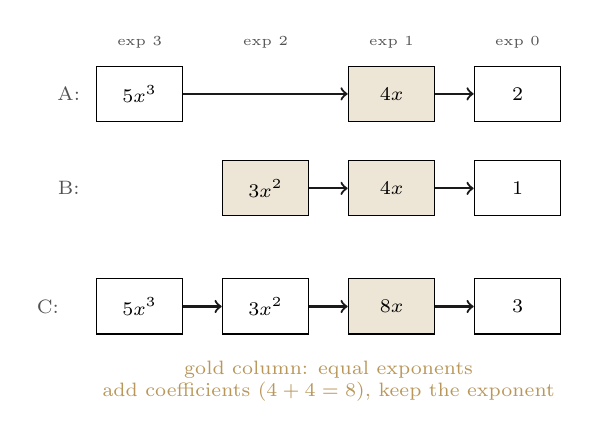
\begin{tikzpicture}[every node/.style={font=\scriptsize}]
    \node[draw, fill=white, minimum width=1.1cm, minimum height=0.7cm,
      align=center] (a3) at (0, 1.5) {$5x^{3}$};
    \node[draw, fill=primary-gold!25, minimum width=1.1cm,
      minimum height=0.7cm, align=center] (a1) at (3.2, 1.5) {$4x$};
    \node[draw, fill=white, minimum width=1.1cm, minimum height=0.7cm,
      align=center] (a0) at (4.8, 1.5) {$2$};
    \draw[->, thick, color=jet] (a3.east) -- (a1.west);
    \draw[->, thick, color=jet] (a1.east) -- (a0.west);

    \node[draw, fill=primary-gold!25, minimum width=1.1cm,
      minimum height=0.7cm, align=center] (b2) at (1.6, 0.3) {$3x^{2}$};
    \node[draw, fill=primary-gold!25, minimum width=1.1cm,
      minimum height=0.7cm, align=center] (b1) at (3.2, 0.3) {$4x$};
    \node[draw, fill=white, minimum width=1.1cm, minimum height=0.7cm,
      align=center] (b0) at (4.8, 0.3) {$1$};
    \draw[->, thick, color=jet] (b2.east) -- (b1.west);
    \draw[->, thick, color=jet] (b1.east) -- (b0.west);

    \node[draw, fill=white, minimum width=1.1cm, minimum height=0.7cm,
      align=center] (c3) at (0, -1.2) {$5x^{3}$};
    \node[draw, fill=white, minimum width=1.1cm, minimum height=0.7cm,
      align=center] (c2) at (1.6, -1.2) {$3x^{2}$};
    \node[draw, fill=primary-gold!25, minimum width=1.1cm,
      minimum height=0.7cm, align=center] (c1) at (3.2, -1.2) {$8x$};
    \node[draw, fill=white, minimum width=1.1cm, minimum height=0.7cm,
      align=center] (c0) at (4.8, -1.2) {$3$};
    \draw[->, thick, color=jet] (c3.east) -- (c2.west);
    \draw[->, thick, color=jet] (c2.east) -- (c1.west);
    \draw[->, thick, color=jet] (c1.east) -- (c0.west);

    \node[text=neutral] at (-0.9, 1.5) {A:};
    \node[text=neutral] at (-0.9, 0.3) {B:};
    \node[text=neutral, anchor=east] at (-0.9, -1.2) {C:};
    \node[text=neutral] at (0, 2.15) {\tiny exp 3};
    \node[text=neutral] at (1.6, 2.15) {\tiny exp 2};
    \node[text=neutral] at (3.2, 2.15) {\tiny exp 1};
    \node[text=neutral] at (4.8, 2.15) {\tiny exp 0};
    \node[text=primary-gold, align=center] at (2.4, -2.15)
      {gold column: equal exponents\\add coefficients ($4 + 4 = 8$), keep
      the exponent};
  \end{tikzpicture}
  \caption{Adding $A = 5x^{3} + 4x + 2$ and $B = 3x^{2} + 4x + 1$ by descending exponent: shared (gold) exponents add coefficients; unshared terms copy through.}
  \label{fig:poly-add}
\end{figure}

\begin{example}[Worked example: add $A = 5x^{3} + 4x + 2$ and $B = 3x^{2} + 4x + 1$]
Walk the merge step by step, tracking \texttt{C} so far:

\begin{center}
{\small
\begin{tabular}{llll}
  \toprule
  \textbf{step} & \textbf{compare} & \textbf{action} & \textbf{C so far} \\
  \midrule
  1 & $3$ vs.\ $2$ & A's exp larger & $5x^{3}$ \\
  2 & $1$ vs.\ $2$ & B's exp larger & $5x^{3} + 3x^{2}$ \\
  3 & $1$ vs.\ $1$ & equal: $4 + 4$ & $5x^{3} + 3x^{2} + 8x$ \\
  4 & $0$ vs.\ $0$ & equal: $2 + 1$ & $5x^{3} + 3x^{2} + 8x + 3$ \\
  \bottomrule
\end{tabular}}
\end{center}

Read the compare column: at each step the larger exponent is copied through, and equal exponents are added. No term is dropped and no zero term is stored. A cancellation (say $4x + (-4x)$) would append \emph{nothing} --- the sparsity discipline in action.

\key{Multiplication} repeats the idea: each term of \texttt{A} times every term of \texttt{B} (coefficients multiply, exponents add), then the resulting terms are merged equal-exponent by equal-exponent --- $O(n \cdot m)$ worst case for $n$ terms of \texttt{A} and $m$ terms of \texttt{B}. \key{Verdict}: the array wins on a small, dense exponent range ($O(1)$ term lookup by exponent); the list wins on a sparse, high-degree polynomial. State the workload, then choose.
\end{example}

\section{Unit-II Review and Close}

\textbf{Read alongside:} Karumanchi, Ch.~3, pp.74--162 (PDF) --- linked lists, the spine of Unit~II (this review is the deck's own, not a new citation).

Unit~II in one map, built for Class Test~2:

\begin{center}
{\footnotesize
\begin{tabular}{@{}p{1.0cm} p{5.2cm} p{5.2cm}@{}}
  \toprule
  \textbf{week} & \textbf{contract} & \textbf{load-bearing skill} \\
  \midrule
  6 & singly list: \texttt{head}, \texttt{p->next}, \texttt{NULL} &
    pointer surgery; three-pointer reverse \\
  7 & DLL \texttt{p->prev}; rings; list stack/queue; polynomials &
    two-link invariant; ring termination; ADT reuse; merge \\
  \bottomrule
\end{tabular}}
\end{center}

The decision array-versus-list is now a full comparison rather than ``lists are better'': positional reads favour the array; anywhere-edits and unpredictable size favour the chain. The test rewards traces --- draw the chain, move the pointers, then name the operation, the bound, and the case.

Three classic mistakes, stated exactly as the deck states them. \bad{Forgetting half the invariant} --- updating \texttt{p->next} but not \texttt{p->next->prev} (or the reverse). The two links silently disagree, and a later backward walk corrupts or skips nodes. \bad{Waiting for \texttt{NULL} in a ring} --- \texttt{while (p != NULL)} on a circular list never terminates; the stop condition must name \texttt{head}. \bad{Ignoring the endpoints} --- forgetting to move \texttt{head} (or clear \texttt{tail}) when the first or last node leaves, or reusing a pointer after \texttt{free}. This is Week~1's dangling pointer and leak, now wearing list clothing. How to revise: re-trace insert-after and delete-by-pointer with a covered answer column, then trace one polynomial addition --- the test is traces, not definitions.

In summary: \key{doubly linked list} --- node $=$ data $+$ \texttt{prev} $+$ \texttt{next}; delete and insert by a known pointer are $O(1)$ worst case, paid for with an extra pointer per node and a two-link invariant to maintain. \key{circular list} --- \texttt{last->next == head}, no \texttt{NULL}; traversal stops at \texttt{head}; singly and doubly rings for round-robin use, and a linked circular queue over a ring. \key{ADT reuse} --- the same Week~3 stack and Week~5 queue contracts run on chains, with $O(1)$ worst-case ends and unbounded size. \key{polynomials} --- ordered $(\text{coeff}, \text{exp})$ nodes; addition is a linear merge by descending exponent; lists win on sparse polynomials, arrays on dense ones. Next week: searching --- linear versus binary, and the elementary sorts that put data in the order binary search needs.

\begin{example}[Before-you-go predictions, with the deck's answers]
Answer from the algorithms, then check in the lab (P7). (1) A DLL holds \texttt{head} $\leftrightarrow$ 5 $\leftrightarrow$ 15 $\leftrightarrow$ 25; delete the node holding 15 given only a pointer to it: the two links rewritten are 5's \texttt{next} $=$ 25 and 25's \texttt{prev} $=$ 5, then \texttt{free} the 15-node --- $O(1)$ worst case. (2) A singly circular list reads a $\to$ b $\to$ c $\to$ a: \texttt{a->next} $=$ b and \texttt{c->next} $=$ a $=$ \texttt{head}; the sentinel that replaces \texttt{NULL} is \texttt{head} itself --- no \texttt{NULL}. (3) Add $(2x^{2} + 1)$ and $(-2x^{2} + 5x)$: the result is $5x + 1$, because the $x^{2}$ terms cancel to coefficient $0$ and a zero term is never stored, while the unshared $5x$ copies through.
\end{example}

\subsection*{Exercises}

Answer from the algorithms, then check against the Solutions block: pointer surgery is Lab work, but every trace below runs on paper first.
\begin{enumerate}
  \item DLL insert trace: start from \texttt{head} $\leftrightarrow$ 10 $\leftrightarrow$ 30. Insert 20 after the 10-node. Give the four pointer writes in order, the final chain, and the two invariant equalities that must hold.
  \item DLL delete trace: on \texttt{head} $\leftrightarrow$ 5 $\leftrightarrow$ 15 $\leftrightarrow$ 25, delete the head node (5) and then the tail node (25). For each, write the bypass assignments (including the \texttt{head} move) and state the cost.
  \item Circular traversal: a singly circular list reads \texttt{head} $\to$ 1 $\to$ 2 $\to$ 3 $\to$ \texttt{head}. What does \texttt{while (p != NULL)} do, and what is the correct terminating loop that prints \texttt{1 2 3} exactly once?
  \item Linked queue: from \texttt{head} $\to$ 10 $\to$ 20 $\to$ 30 $\to$ \texttt{NULL} with \texttt{tail} at 30, run \texttt{dequeue()} twice, then \texttt{enqueue(40)}. Give the chain and the location of \texttt{head} and \texttt{tail} after each operation, and say why the \texttt{if (head == NULL) tail = NULL} guard matters. (Genuinely new instance reusing the deck's two-end pattern.)
  \item Polynomial addition: add $A = 4x^{4} + 2x^{2} + 7$ and $B = 3x^{3} + 2x^{2} + 5$. Give the step-by-step merge, the final chain in descending exponent order, and the worst-case time bound. Which terms, if any, are cancelled?
\end{enumerate}

\subsection*{Solutions}

\begingroup\small
\begin{enumerate}
  \item \textbf{Writes: (1) \texttt{X->next = p->next} (30); (2) \texttt{X->prev = p} (10); (3) \texttt{30->prev = X}; (4) \texttt{10->next = X}. Final chain: \texttt{head} $\leftrightarrow$ 10 $\leftrightarrow$ 20 $\leftrightarrow$ 30. Invariant: \texttt{20->next->prev} $=$ \texttt{30->prev} $=$ 20 and \texttt{20->prev->next} $=$ \texttt{10->next} $=$ 20.} Step~3 is guarded by \texttt{p->next != NULL} (here 30 exists); step~4 must come after step~3, which still needs the old successor value.
  \item \textbf{Delete 5 (head): \texttt{p->prev == NULL}, so \texttt{head = p->next} (the 15-node); then \texttt{15->prev = NULL}; \texttt{free(p)}. Delete 25 (tail): \texttt{25->prev} is 15, so \texttt{15->next = p->next} $=$ \texttt{NULL}; then \texttt{p->next == NULL}, so no backward repair; \texttt{free(p)}. $O(1)$ worst case each once \texttt{p} is in hand.} Both bypasses are $O(1)$; skipping either free leaks one box, and touching \texttt{p} after is the dangling pointer.
  \item \textbf{\texttt{while (p != NULL)} loops forever: no \texttt{next} is \texttt{NULL} in a ring, so the test never fires. Correct loop: \texttt{p = head; if (p != NULL) do \{ print p->data; p = p->next; \} while (p != head);} --- the \texttt{do--while} visits \texttt{head} first and stops when the walk returns to it, printing \texttt{1 2 3} once.} A plain \texttt{while (p != head)} would skip node 1 (the head), hence the \texttt{do--while} form.
  \item \textbf{After dequeue 1: \texttt{head} $\to$ 20 $\to$ 30 $\to$ \texttt{NULL}, \texttt{tail} at 30. After dequeue 2: \texttt{head} $\to$ 30 $\to$ \texttt{NULL}, \texttt{tail} still 30. After enqueue 40: \texttt{head} $\to$ 30 $\to$ 40 $\to$ \texttt{NULL}, \texttt{tail} at 40.} The guard matters when the queue empties: removing the final item sets \texttt{head} $=$ \texttt{NULL}, and \texttt{tail} must follow to \texttt{NULL} or the next enqueue writes through a stale pointer into freed memory.
  \item \textbf{Merge: compare 4 vs.\ 3 $\to$ copy $4x^{4}$; 2 vs.\ 3 $\to$ copy $3x^{3}$; 2 vs.\ 2 $\to$ $2+2=4$, emit $4x^{2}$; A has $7$, B has $5$, both exp 0 $\to$ $7+5=12$, emit $12$. Final chain: \texttt{(4,4)} $\to$ \texttt{(3,3)} $\to$ \texttt{(4,2)} $\to$ \texttt{(12,0)} $\to$ \texttt{NULL}, i.e.\ $4x^{4} + 3x^{3} + 4x^{2} + 12$. No term cancels here (all sums nonzero); worst-case time $O(n+m)$ } The merge visits each source node once and emits at most one output node per step; the equal-exponent step adds coefficients ($2+2$, $7+5$) and keeps the exponent.
\end{enumerate}
\endgroup

\bibliography{../../Bibliography_base}
\bibliographystyle{plain}
\end{document}
